\chapter{Συστήματα Συντεταγμένων}
\label{apx:coordinates}

\section{Καρτεσιανές συντεταγμένες}
Cartesian coordinates allow one to specify the location of a point in the plane, or in three-dimensional space. The Cartesian coordinates (also called rectangular coordinates) of a point are a pair of numbers (in two-dimensions) or a triplet of numbers (in three-dimensions) that specified signed distances from the coordinate axis.

\subsection{Καρτεσιανές συντεγαμένες στο επίπεδο}
The Cartesian coordinates in the plane are specified in terms of the x coordinates axis and the y-coordinate axis, as illustrated in the below figure (Σχήμα \ref{fig:apxA_cartesian2D}). The origin is the intersection of the x and y-axes. The Cartesian coordinates of a point in the plane are written as (x,y). The first number x is called the x-coordinate (or x-component), as it is the signed distance from the origin in the direction along the x-axis. The x-coordinate specifies the distance to the right (if x is positive) or to the left (if x is negative) of the y-axis. Similarly, the second number y is called the y-coordinate (or y-component), as it is the signed distance from the origin in the direction along the y-axis, The y-coordinate specifies the distance above (if y is positive) or below (if y is negative) the x-axis. The following figure, the point has coordinates (-3,2), as the point is three units to the left and two units up from the origin.

\begin{figure}[h]
    \centering
    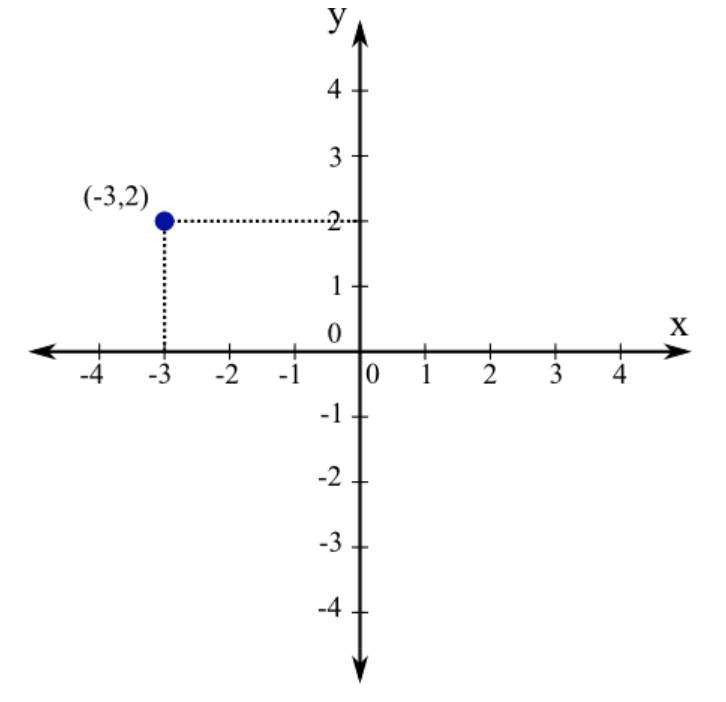
\includegraphics[scale=0.5]{Figures/appendixA_cartesian2D.png}
    \caption{Καρτεσιανές συντεταγμένες στο επίπεδο. The Cartesian coordinates (x,y) of the blue point specify its location relative to the origin, which is the intersection of the x- and y-axis.}
    \label{fig:apxA_cartesian2D}
\end{figure}


\subsection{Καρτεσιανές συντεταγμένες στον χώρο}
In three-dimensional space, the Cartesian coordinate system is based on three mutually perpendicular coordinate axes: the x-axis, the y-axis, and the z-axis, illustrated below. The three axes intersect at the point called the origin. You can imagine the origin being the point where the walls in the corner of a room meet the floor. The x-axis is the horizontal line along which the wall to your left and the floor intersect. The y-axis is the horizontal line along which the wall to your right and the floor intersect. The z-axis is the vertical line along which the walls intersect.

\begin{figure}[h]
    \centering
    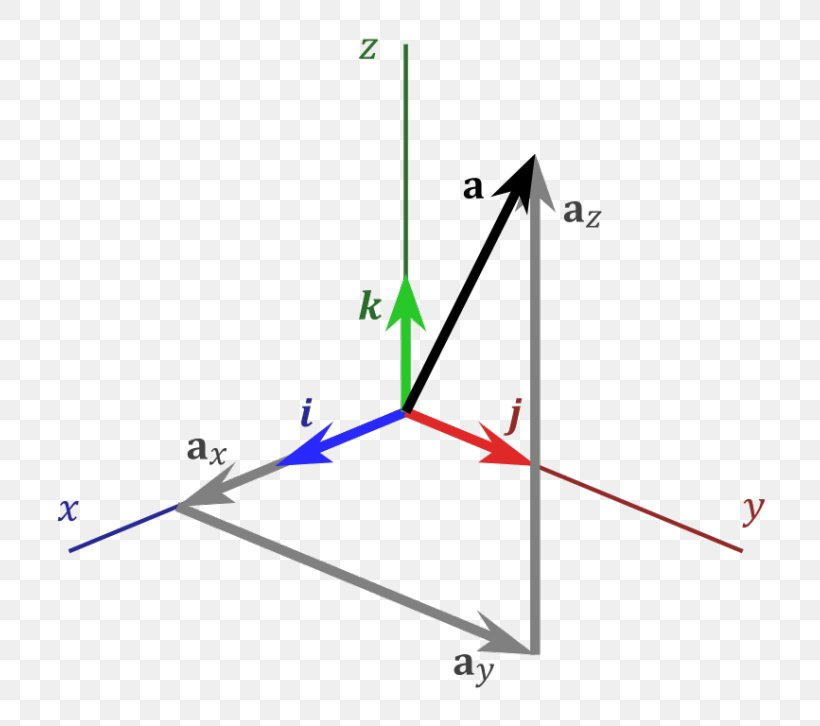
\includegraphics[scale=0.3]{Figures/appendixA_cartesian3D.jpg}
    \caption{Καρτεσιανές συντεταγμένες στον χώρο.}
    \label{fig:apxA_cartesian3D}
\end{figure}

With above definitions of the positive x, y, and z-axis, the resulting coordinate system is called right-handed; if you curl the fingers of your right hand from the positive x-axis to the positive y-axis, the thumb of your right hand points in the direction of the positive z-axis. Switching the locations of the positive x-axis and positive y-axis creates left-handed coordinate system. The right-handed and left-handed coordinate systems represent two equally valid mathematical universes. The problem is that switching universes will change the sign on some formulas. Since these pages are written in the right-handed universe, we suggest you live in our universe while studying from these pages.

In addition to the three coordinate axes, we often refer to three coordinate planes. The xy-plane is the horizontal plane spanned by the x and y-axes. It is identical to the two-dimensional coordinate plane and contains the floor in the room analogy. Similarly, the xz-plane is the vertical plane spanned by the x and z-axes and contains the left wall in the room analogy. Lastly, the yz-plane is the vertical plane spanned by the y and the z-axis and contains the right wall in the room analogy.
\\
{\color{red} \hrule}
Cartesian coordinates can be used not only to specify the location of points, but also to specify the coordinates of vectors. The Cartesian coordinates of two or three-dimensional vectors look just like those of points in the plane or three-dimensional space.

Από το σχήμα \ref{fig:apxA_cartesian3D} προκύπτει ότι το διάνυσμα θέσεως ,$\boldsymbol{a}$, θα δίνεται από τη σχέση: $$\boldsymbol{a} = a_x \boldsymbol{i} + a_y \boldsymbol{j} + a_z \boldsymbol{k}$$

But, there is no reason to stop at three-dimensions. We could define vectors in four, five, or higher dimensions by just specifying four, five, or more Cartesian coordinates. We can't visualize these higher dimensions like we did with the above applets, but we can easily write down the list of numbers for the coordinates.\\
{\color{red} \hrule}


\section{Πολικές συντεταγμένες}
In two dimensions, the Cartesian coordinates (x,y) specify the location of a point P in the plane. Another two-dimensional coordinate system is polar coordinates. Instead of using the signed distances along the two coordinate axes, polar coordinates specifies the location of a point P in the plane by its distance r from the origin and the angle $\theta$ made between the line segment from the origin to P and the positive x-axis. The polar coordinates $(r, \theta)$ of a point P are illustrated in the below figure (Σχήμα \ref{fig:apxA_polar_coordinates}).

\begin{figure}[h]
   \centering
\begin{subfigure}[h]{0.45\textwidth}
	\centering
   	 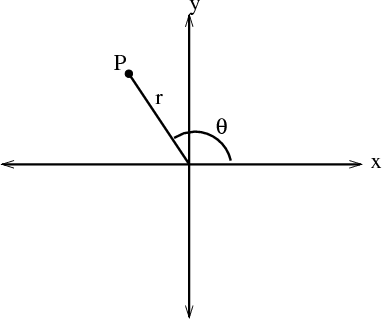
\includegraphics[width = \linewidth]{Figures/appendixA_polar_coordinates_whole.png} 
\end{subfigure}
\begin{subfigure}[h]{0.4\textwidth}
	\centering
	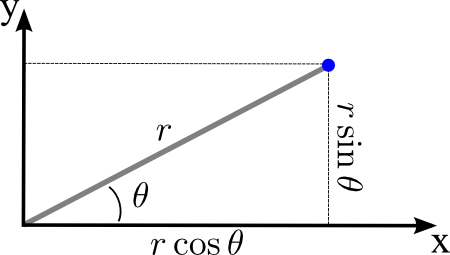
\includegraphics[width = \linewidth]{Figures/appendixA_polar_coordinates.png} 
    \end{subfigure}
    \caption{Πολικές συντεταγμένες στο επίπεδο.}
    \label{fig:apxA_polar_coordinates}
\end{figure}

As r ranges from 0 to infinity and $\theta$ ranges from 0 to $2\pi$, the point P specified by the polar coordinates $(r, \theta)$ covers every point in the plane. Adding $2\pi$ to $\theta$ brings us back to the same point, so if we allowed $\theta$ to range over an interval larger than $2\pi$, each point would have multiple polar coordinates. Hence, we typically restrict $\theta$ to be in the interval $0\leq \theta \leq 2\pi$. However, even with that restriction, there still is some non-uniqueness of polar coordinates: when $r=0$, the point P is at the origin independent of the value of $\theta$.

We can calculate the Cartesian coordinates of a point with polar coordinates $(r, \theta)$ by forming the right triangle illustrated in Figure \ref{fig:apxA_polar_coordinates}.  The hypotenuse is the line segment from the origin to the point, and its length is r. The projection of this line segment on the x-axis is the leg of the triangle adjacent to the angle $\theta$, so $x=r \cos \theta$. The y-component is determined by the other leg, so $y = r \sin \theta$. Our conversion formula is:
\begin{eqnarray}
    x &=& r \cos \theta \\
    y &=& r \sin \theta 
\end{eqnarray}

Για τους αντίστροφους μετασχηματισμούς προκύπτει από τις παραπάνω σχέσεις ότι:
\begin{eqnarray}
    x^2 + y^2 &=& r^2 (\cos^2 \theta + \sin^2 \theta) = r^2 \Rightarrow r = \sqrt{x^2 + y^2} \\ \nonumber \\
    \frac{y}{x} &=& \frac{r \sin \theta}{r \cos \theta} = \tan \theta \Rightarrow \theta = \arctan \left( \frac{y}{x} \right)
\end{eqnarray}

Παρατηρούμε ότι με βάση τη σχέση Α.4 για το σημείο $(x,y) = (0,0)$, η γωνία $\theta$ δεν ορίζεται. Σε αυτή την περίπτωση όμως παίρνουμε ότι $\theta = 0$.


\section{Κυλινδρικές συντεταγμένες}
Cylindrical coordinates are a simple extension of the two-dimensional polar coordinates to three dimensions. They simply combine the polar coordinates in the xy-plane with the usual z coordinate of Cartesian coordinates. To form the cylindrical coordinates of a point P, simply project it down to a point Q in the xy-plane (Σχήμα \ref{fig:apxA_cylindrical_coordinates}). Then, take the polar coordinates $(r, \theta)$ of the point Q, i.e., r is the distance from the origin to Q and $\theta$ is the angle between the positive x-axis and the line segment from the origin to Q. The third cylindrical coordinate is the same as the usual z-coordinate. It is the signed distance of the point P to the xy-plane (being negative is P is below the xy-plane). The below figure illustrates the cylindrical coordinates $(r, \theta, z)$ of the point P.

\begin{figure}[h]
    \centering
    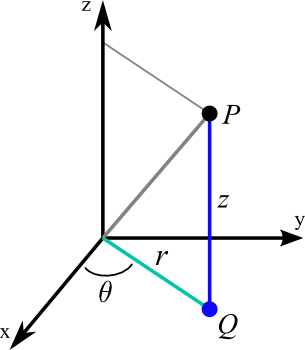
\includegraphics[scale=0.5]{Figures/appendixA_cylindrical_coordinates.png}
    \caption{Κυλινδρικές συντεταγμένες στον χώρο.}
    \label{fig:apxA_cylindrical_coordinates}
\end{figure}

Οι μετασχηματισμοί δίνονται από τις σχέσεις:
\begin{eqnarray}
    x &=& r \cos \theta \\
    y &=& r \sin \theta \\
    z &=& z
\end{eqnarray}
ενώ για τους αντίστροφους μετασχηματισμούς, ισχύουν οι σχέσεις Α.3 και Α.4.

\section{Σφαιρικές συντεταγμένες}
Spherical coordinates can be a little challenging to understand at first. Spherical coordinates determine the position of a point in three-dimensional space based on the distance $\rho$ from the origin and two angles $\theta$ and $\phi$. If one is familiar with polar coordinates, then the angle $\theta$ isn't too difficult to understand as it is essentially the same as the angle $\theta$ from polar coordinates. But some people have trouble grasping what the angle $\phi$ is all about\footnote{Όλο το παράρτημα είναι μετάφραση της σελίδας \url{https://mathinsight.org/spherical_coordinates}, η οποία περιέχει και διάφορα applets για την καλύτερη κατανόηση των εννοιών.}. Στη συνέχεια θα εξάγουμε τις σχέσεις μεταξύ Καρτεσιανών και σφαιρικών συντενταγμένων.

Οι σφαιρικές συντεταγμένες ορίζονται βάσει του σχήματος \ref{fig:apxA_spherical_coordinates}, το οποίο δείχνει τις σφαιρικές συντεταγμένες στο σημείο P.

\begin{figure}[h]
    \centering
    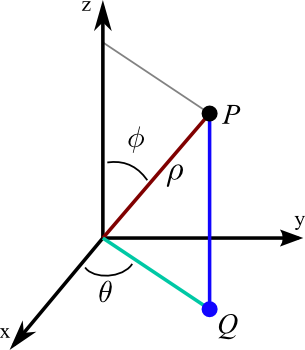
\includegraphics[scale=0.5]{Figures/appendixA_spherical_coordinates_simple.png}
    \caption{Σφαιρικές συντεταγμένες στον χώρο.}
    \label{fig:apxA_spherical_coordinates}
\end{figure}

The coordinate $\rho$ is the distance from P to the origin. If the point Q is the projection of P to the xy-plane, then $\theta$ is the angle between the positive x-axis and the line segment from the origin to Q. Lastly, $\phi$ is the angle between the positive z-axis and the line segment from the origin to P.

We can calculate the relationship between the Cartesian coordinates $(x, y, z)$ of the point P and its spherical coordinates $(\rho, \theta, \phi)$ using trigonometry. Το ροζ τρίγωνο του Σχήματος \ref{fig:apxA_spherical_coordinates_derivation} is the right triangle whose vertices are the origin, the point P, and its projection onto the z-axis. As the length of the hypotenuse is $\rho$ and $\phi$ is the angle the hypotenuse makes with the z-axis leg of the right triangle, the z-coordinate of P (i.e., the height of the triangle) is $z = \rho \cos \phi$. The length of the other leg of the right triangle is the distance from P to the z-axis, which is $r = \rho \sin \phi$. The distance of the point Q from the origin is the same quantity.

\begin{figure}[h]
    \centering
    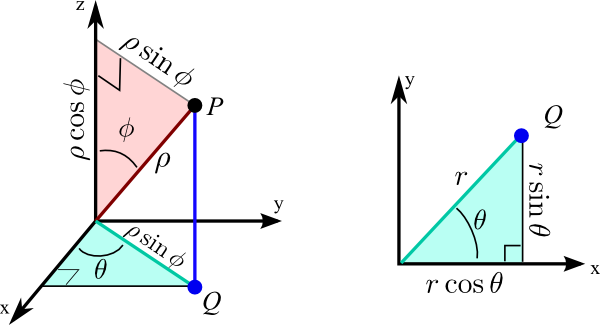
\includegraphics[scale=0.5]{Figures/appendixA_spherical_coordinates_analytical.png}
    \caption{Σχέση Καρτεσιανών και σφαιρικών συντενταγμένων.}
    \label{fig:apxA_spherical_coordinates_derivation}
\end{figure}

The cyan triangle, shown in both the original 3D coordinate system on the left and in the xy-plane on the right, is the right triangle whose vertices are the origin, the point Q, and its projection onto the x-axis. In the right plot, the distance from Q to the origin, which is the length of hypotenuse of the right triangle, is labeled just as r. As $\theta$ is the angle this hypotenuse makes with the x-axis, the x- and y-components of the point Q (which are the same as the x- and y-components of the point P) are given by $x = r \cos \theta$ and $y = r \sin \theta$. Since $r = \rho \sin \phi$, these components can be rewritten as $x = \rho \sin \phi \cos \theta$ and $y = \rho \sin \phi \sin \theta$. In summary, the formulas for Cartesian coordinates in terms of spherical coordinates are:

\begin{eqnarray}
    x &=& \rho \sin \phi \cos \theta \\
    y &=& \rho \sin \phi \sin \theta \\
    z &=& \rho \cos \phi
\end{eqnarray}
όπου $\rho \geq 0, 0 \leq \theta \leq 2\pi, 0 \leq \phi \leq \pi$.

Unfortunately, the convention for the notation of spherical coordinates is not standardized across disciplines. For example, in physics, the roles of $\theta$ and $\phi$ are typically reversed. In order to correctly understand someone's use of spherical coordinates, you must first determine what notational convention this are using. You cannot assume they follow the convention used here.
